\chapter{Background} \label{chapter:background}


\section{Existing Applications}

% overview

There are a number of existing applications available that attempt to solve the problem posed by this project. These range from fitness applications to various navigation applications, which although may not be completely relevant to this project, do provide some similar features such as place recognition that will be useful to research.

Table \ref{table:existing-walking-apps} shows how well each of the existing applications related to this project have implemented certain features. The maximum score for the feature category is displayed in brackets. The full matrix detailing what aspects each feature category is split into and why the score was given to each app can be seen in Appendix \ref{appendix:existing-apps-matrices}.

\begin{table}[htb]
  \centering
  \begin{tabular}{|m{2cm}||c|c|M{1.5cm}|M{1.5cm}|c|c|}
    \hline
    \textbf{Features} & \textbf{MapMyWalk} & \textbf{Strava} & \textbf{Let's Walk} & \textbf{Google Maps} & \textbf{Citymapper} & \textbf{Pok\'{e}mon Go}\\
    \hline
    \hline
    Design (2) & 2 & 2 & 2 & 2 & 2 & 2\\
    \hline
    Ease of use (3) & 3 & 3 & 2 & 3 & 3 & 3\\
    \hline
    Tracking location (2) & 2 & 2 & 2 & 1 & 1 & 1\\
    \hline
    Navigation (4) & 3 & 1 & 1 & 3 & 1 & 2\\
    \hline
    Social interaction (5) & 2 & 2 & 2 & 0 & 0 & 0\\
    \hline
    \hline
    Total (16) & 12 & 10 & 9 & 8 & 7 & 9\\
    \hline
  \end{tabular}  
  \caption{Matrix showing how well existing walking apps perform at given features. Each app is given a score for a category, with the maximum score shown in brackets next to the feature category.}
  \label{table:existing-walking-apps}
\end{table}

The rest of this section discusses each application in detail, explaining their benefits and limitations. All of the applications researched are free to use unless stated otherwise.

% go through each existing app, discussing why they are good/bad with images

\subsection{MapMyWalk}

MapMyWalk \cite{Map} is a popular fitness application for iOS and Android that allows you to track your walks and compete against other users by completing challenges. You are able to track a walk as you go on one, or log a previous workout that you have done without the app.

The app also provides a premium subscription for \pounds4.49 per month, which gives you the ability to monitor your heart rate and set training goals designed to help you walk more.

\subsection{Strava}

Strava \cite{StravaInc.} is another fitness application that primarily focuses on running and cycling. It features a sleek user interface with similar functionalities as MapMyWalk. The journey view within the application can switch between either showing the map of your workout or a statistics screen as shown in Figure \ref{fig:strava}, visibly showing the time elapsed in the workout, the distance travelled and your average pace per kilometre.

The setback of Strava is that you cannot track walks in the app, you are constrained to either running or cycling. 

\begin{figure}[hbt]
  \centering
  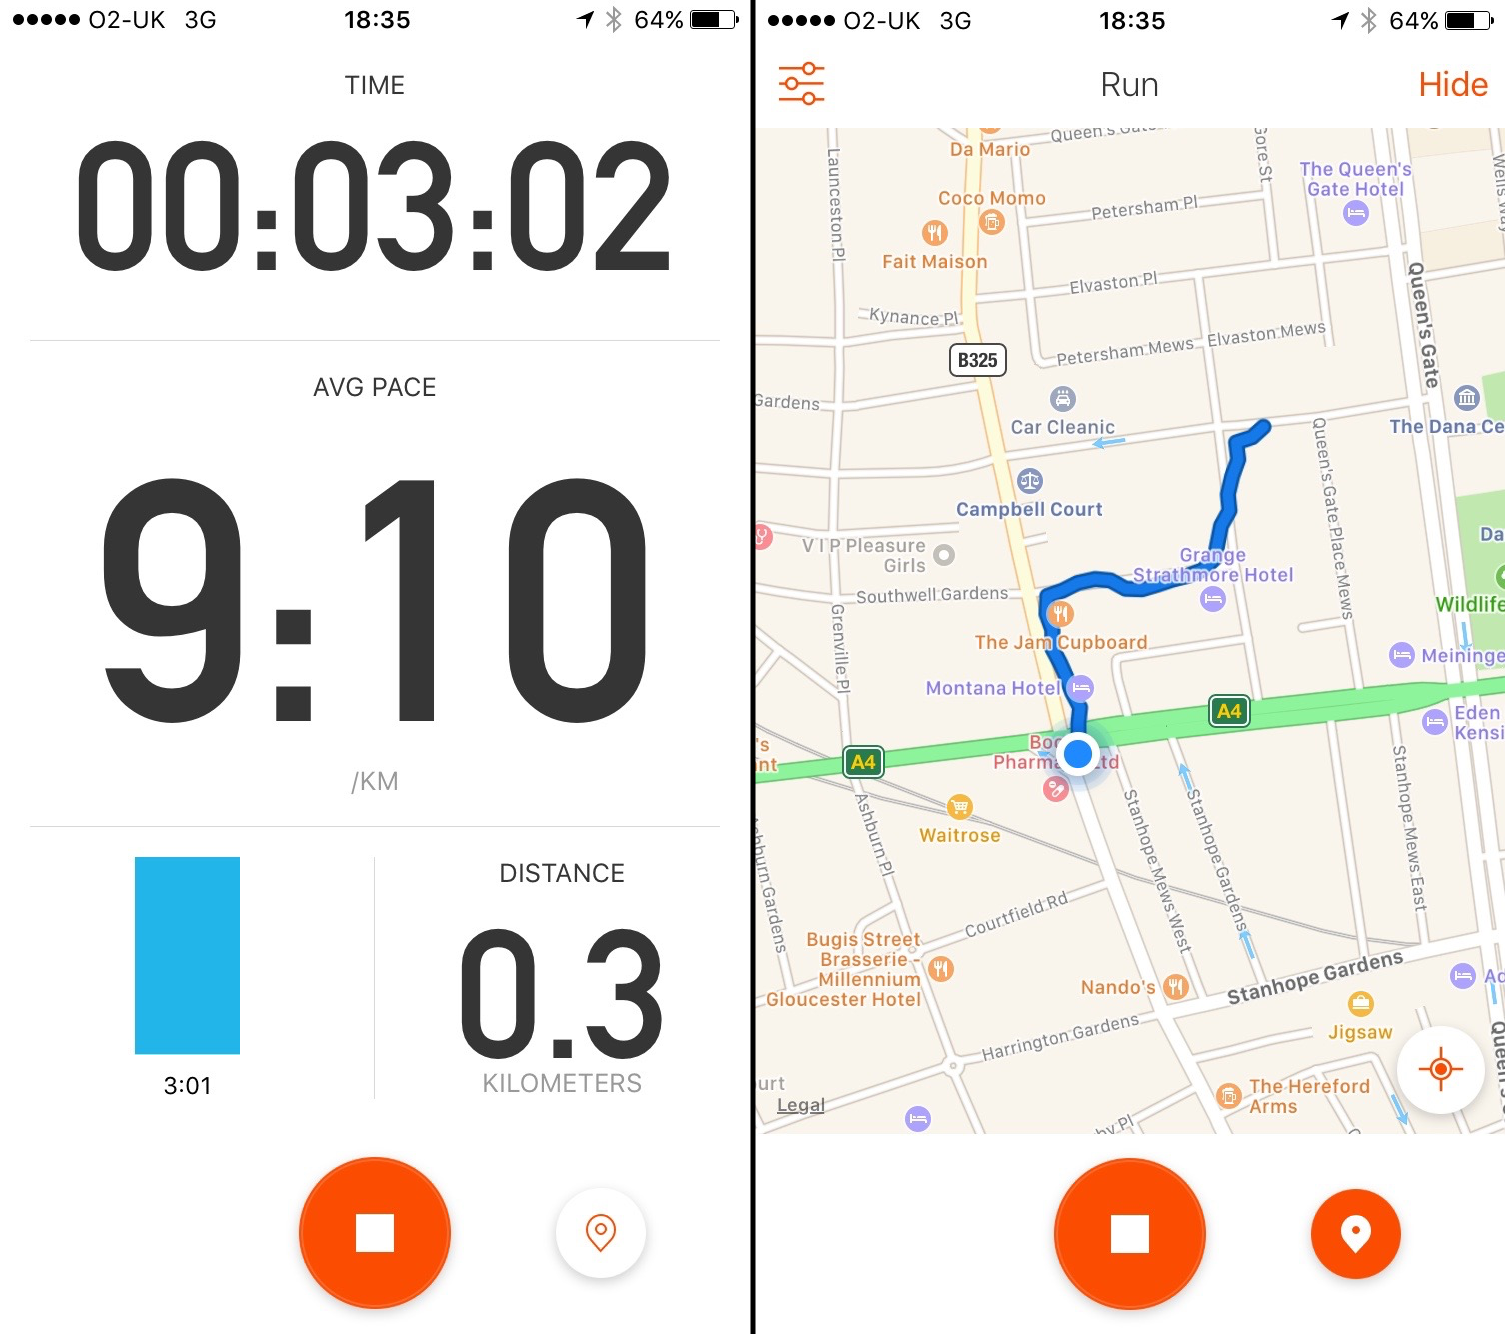
\includegraphics[width=0.8\textwidth]{strava}
  \caption{Journey view in Strava, allowing you to switch between statistics (left) or a map of your progress (right)}
  \label{fig:strava}
\end{figure}


\subsection{Let's Walk}

A lesser well-known iOS application is Let's Walk \cite{LetsWalkApp}. Users can record new walks and view a list of either their friends' walks or public walks nearby. It tries to emulate many of the features implemented by the bigger apps as mentioned above, but a lot of these features seem unpolished. There is a global ranking section of the application showing which users have walked the most over the last week, month or year, however there seems to be little to do with this information other than view a leaderboard.

The app is also focused on helping you maintain a balanced diet -- the amount of calories consumed can be added for particular meals during the day. A calorie goal per day can then be added, with the app recording how many calories were burned during a walk and updating the goal accordingly.

\subsection{Google Maps}

Although not a fitness application per say, Google Maps \cite{GoogleInc.} is one of the oldest services that provides route planning via different transport modes. The app contains current information about public transport, traffic and displays well-known cycling routes on map but there is little in the way of customisation for walking. When entering a destination, the app generates a route but users can also choose from a few different routes on map with the difference in time each one would take. However, no information is given as to whether a certain route is quieter than another, for example.

\begin{figure}[hbt]
  \centering
  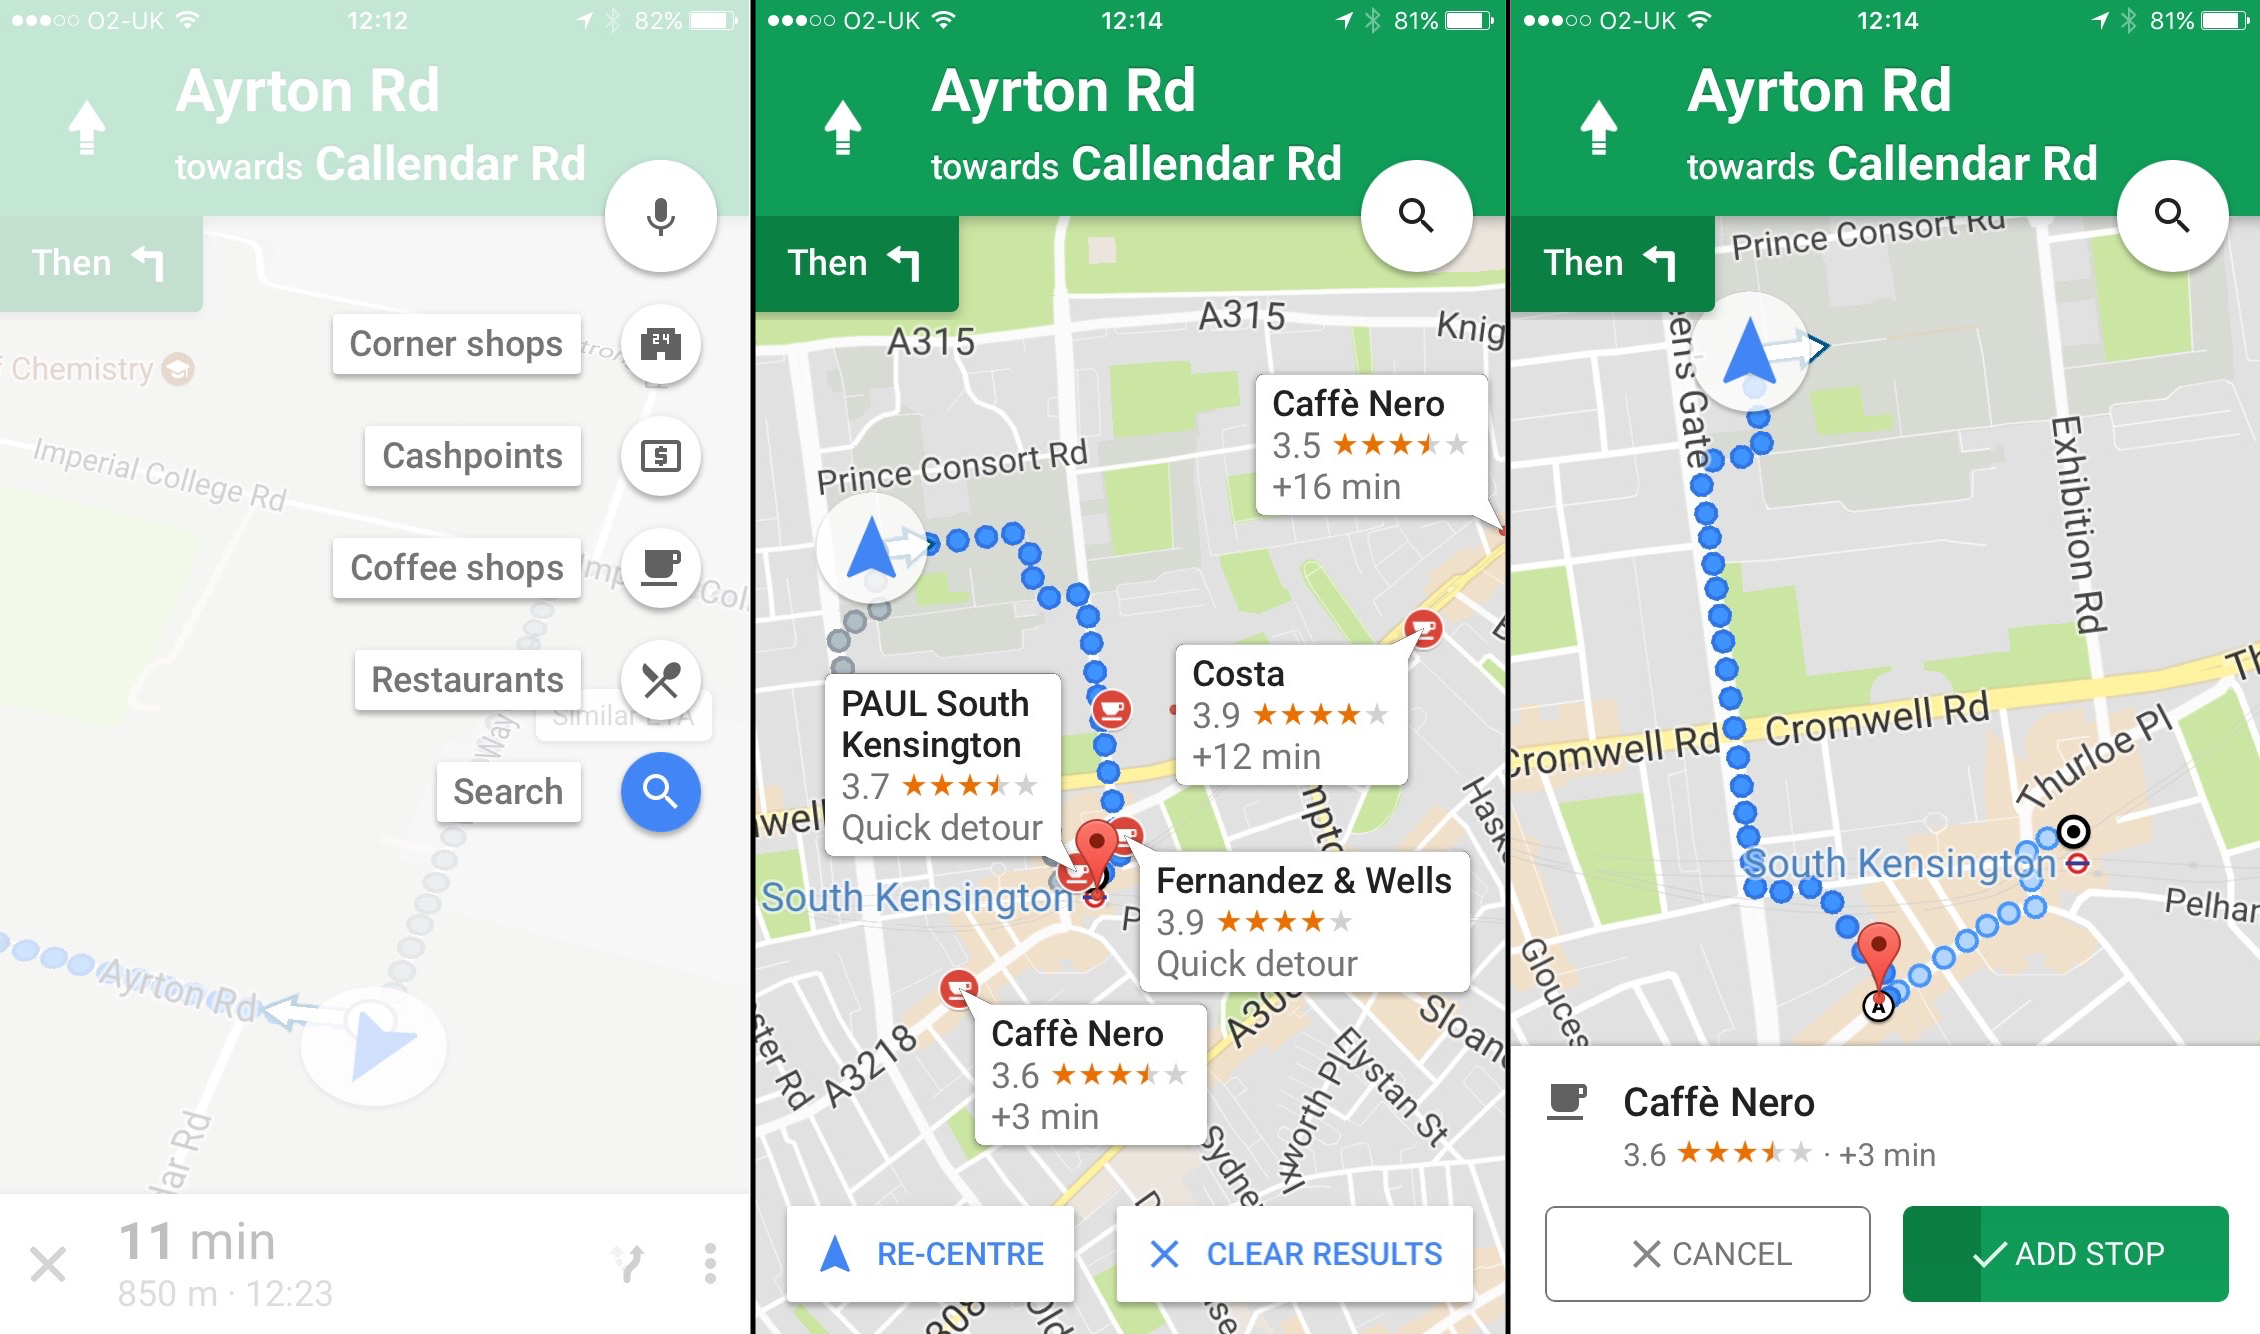
\includegraphics[width=\textwidth]{google_maps_place_search}
  \caption{Adding places along your walking route in Google Maps for iOS. A list of categories to choose from (left), then shows all the places from within a search on a map (middle). A stop can then be added and the journey will be updated (right).}
  \label{fig:google_maps_place_search}
\end{figure}


One feature of the Google Maps iOS application that is interesting to note is the places search along a route during a journey. Once a user has started a walking journey, they are able to search for places that are along the route. Google provides some categories of places to choose from, such as cashpoints and restaurants, but users can search for a specific place if they wish. The app will then display the results of the places search on the map showing how much additional time would be added on to your journey if you were to stop at a place, if any. One of more places can then be added to your journey and the walking directions will subsequently update to include these new stops. Figure \ref{fig:google_maps_place_search} shows an example journey from Imperial College to South Kensington station. It details the full process of choosing \textit{coffee shops} as the place category, selecting a particular coffee shop on the map and the stop being added to the journey.

The places search feature is important as it is unique within any of the existing journey planner apps I have researched and it relates to one of my objectives regarding displaying points of interest when a user is on a walk (\textbf{Obj 3}). More research is conducted in Section *** to discover what tools these applications use to implement this feature.

\subsection{Citymapper}

Originating in London, Citymapper \cite{Citymapper} has become one of the leading journey planners for major cities around the world including Paris, Barcelona, New York, Tokyo and Sydney. One of the key features of Citymapper is that different modes of transport can be combined to create a faster journey time. For example, a journey from Imperial College to Oxford Circus as shown in Figure \ref{fig:citymapper} could just use the Tube, but it could be faster to hire a bike to a different station and then take the Tube.

\begin{figure}[hbt]
  \centering
  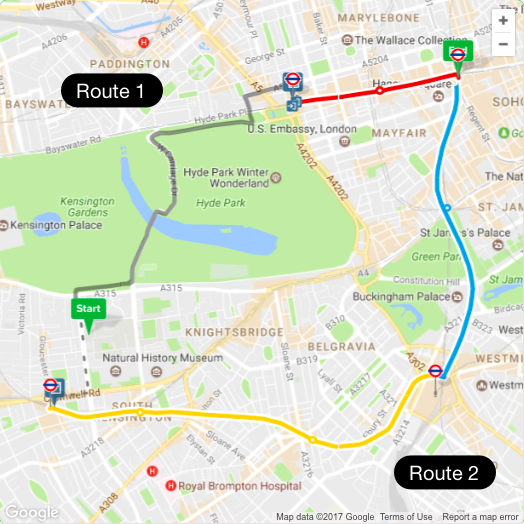
\includegraphics[width=0.7\textwidth]{citymapper}
  \caption{Two routes generated on the Citymapper website superimposed}
  \label{fig:citymapper}
\end{figure}


\subsection{Pok\'{e}mon Go}

%Pok\'{e}mon Go

% maybe don't include this
%Although existing navigation apps do not contain any features relating to tracking walks, they do provide information about how journeys and places are displayed on a map.

\subsection{Summary}

\section{Gamification}

% research how gamification has been used in applications, not just walking apps
% discuss how well each implementation has worked


% not sure whether to include this in background or design?
% think I will include general background on technologies here, and then which ones I chose in design
\section{Technologies}

The features of existing applications are not the only important part to research -- the technologies that they use to implement these features are just as useful. This section discusses how existing applications implement certain features and what technologies integrate well with each other.

\subsection{Operating System}

Many of the applications that I have researched have been developed for iOS, the operating system running on iPhones and iPads. I have chosen to develop my application on iOS due to my previous experience with iOS app development. One of the programming languages that iOS apps are developed in is Swift, which is extremely readable and easy to use.

\subsection{Location Tracking}

To track the user's location within iOS, an application can use the classes from the Core Location framework \cite{AppleInc.} inbuilt into the iOS SDK (software development kit). This framework allows a developer to obtain the user's current location in the form of latitude and longitude. To keep a history of where the user has been, these coordinates could be stored in an array and updated after a certain period of time.

% section on how to track calories burned?

\subsection{APIs}

Map APIs

Places APIs

% compare Google Maps and Apple Maps
% and Google Places etc.
